%!TEX root = main.tex


\section{Probability with connectable submodels}

Throughout this paper, we will assume all measurable sets $X$ are finite sets. This is both because it makes explanations simpler and because it is easy to show that submodels exist in this setting (Lemma \ref{lem:subm_exist}). Many of the proofs in this paper can likely be specialised to more general settings due to our use of string diagrams which represent abstract morphisms in Markov categories, rather than finite Markov kernels specifically.

The standard method of constructing probability models introduces a probability space $(\prob{P},(\Omega,\sigalg{F}))$ with $\Omega$ a sample space, $\sigalg{F}$ a $\sigma$-algebra on $\Omega$ and $\prob{P}$ a probability measure on $(\Omega,\sigalg{F})$. Random variables are defined by measurable functions on $\Omega$ and are given names in sans-serif like $\RV{X}$. A probability distribution $\prob{P}^{\RV{XYZ}}$ is ``the joint distribution of $\RV{X}$, $\RV{Y}$ and $\RV{Z}$ under $\prob{P}$'' where $\RV{X},$ $\RV{Y}$ and $\RV{Z}$ are associated with random variables on $\Omega$ and is given by the pushforward of the function $\omega\mapsto (\RV{X}(\omega),\RV{Y}(\omega),\RV{Z}(\omega))$. Unless otherwise stated, a random variable named $\RV{X}$ will take values in the space $X$ (note the serif font).

This approach needs to be extended if we are to apply it to causal modelling. The causal graphical models literature provides some simple examples illustrating this need, while the fact that the potential outcomes approach also benefits from extension requires more explanation, and will be discussed in Section \ref{sec:potential_outcomes}. 

Consider the ``truncated factorisation'', a linchpin operation in causal graphical models. Given a probability $\prob{P}^{\RV{XYZ}}$ and a graphical model in which $\RV{Z}$ blocks all backdoor paths between $\RV{X}$ and $\RV{Y}$, the truncated factorisation defines a new probability measure $\prob{P}_x$ as follows \citep[page ~24]{pearl_causality:_2009}:
\begin{align}
	\prob{P}^{\RV{YZ}}_{x}(y,z):=\prob{P}^{\RV{Y|XZ}}(y|x,z)\prob{P}^{\RV{Z}}(z)\label{eq:truncated_fac}
\end{align}

Without a causal model justifying the claim that $\RV{Z}$ blocks backdoor paths between $\RV{X}$ and $\RV{Y}$, there is in general no special siginificance to the expression on the right side of Equation \ref{eq:truncated_fac}, and causal models that can justify such claims are not a feature of the standard approach to probability modelling. At the same time, the notation we have chosen for the left side of Equation \ref{eq:truncated_fac} suggests that $\prob{P}^{\RV{YZ}}_{x}$ is a distribution over the same variables $\RV{Y}$ and $\RV{Z}$ as the original $\prob{P}^{\RV{XYZ}}$. The standard approach to probability modelling \emph{does} offer an account of what it means for variables to be the same, which is that they are represented by the same measurable functions on the probability space.

An immediate issue is that $\prob{P}_x$ is a different probability measure to $\prob{P}$. However, even if we substitute probability measures, we could perhaps keep the sample space $\Omega$ and define variables as measurable functions on $\Omega$. This is the approach taken in \citet{pearl_causality:_2009} (but see Section \ref{sec:vague_variables}).

This approach rules out the possibility of performing some interventions. For example, if $\RV{X}=\RV{Z}$ and $\prob{P}^{\RV{Z}}$ is non-deterministic, then no $\prob{P}_x$ exists with the property required in Equation \ref{eq:truncated_fac}. We think that this is probably a useful feature. Consider a variable $\RV{B}$ representing a person's body mass index. It seems reasonable to hold that this variable is by definition equivalent to $\frac{\RV{W}}{\RV{H}^2}$ where $\RV{W}$ represents their weight in kilograms and $\RV{H}$ represents their height in metres. This rules out the existence of any probability measure that represents the results of an intervention on $\RV{B}$ in any model that also contains $\RV{H}$ and $\RV{W}$ and features the expected causal relationships (and, regardless of causal relationships, it completely rules out the possibility that $\RV{B}$, $\RV{H}$ and $\RV{W}$ can all be intervened on). Such interventions can be ruled out by defining the random variables such that $\RV{B} = \frac{\RV{W}}{\RV{H}^2}$.

Along the same lines as \citet{dawid_causal_2000}, we find that it is often desirable to introduce variables representing the results of choices, and we often don't want to attach probability distributions to such variables. We might have $\RV{D}$, representing a choice, and $\prob{P}^{\RV{Y}|\RV{D}}$ representing the consequences of this choice, but no $\prob{P}^{\RV{Y},\RV{D}}$ as we have no need of a marginal probability of $\RV{D}$.

As a brief summary, we want a version of ``probability theory'' that:
\begin{itemize}
	\item Defines what we mean by a ``variable''
	\item Includes generalised variables that do not have marginal probabilities (for example, to represent choices)
	\item Operations like Equation \ref{eq:truncated_fac} are standard rather than special cases
\end{itemize}

Standard probability theory does the first, but not the second two.

\subsection{Markov categories}
We base our approach on the theory of Markov categories. This has two benefits: firstly, Markov categories have a graphical notation that help present some ideas in an intuitive manner. Secondly, because they are abstract categories that represent models of the flow of information, proofs that use only string diagrams correspond to theorems in many formalisations of probability, not just the finite set case that we focus on here. More comprehensive introductions to Markov categories can be found in \citet{fritz_synthetic_2020,cho_disintegration_2019}.

Rather than explain Markov categories in the abstract, we will instead introduce string diagrams with reference to how they represent stochastic maps and finite sets (though see Appendix \ref{sec:app_mcat}). Given measurable sets $(X,\sigalg{X})$ and $(Y,\sigalg{Y})$, a Markov kernel or stochastic map is a map $\kernel{K}:X\times \sigalg{Y}\to [0,1]$ such that

\begin{itemize}
	\item The map $x\mapsto \kernel{K}(x,A)$ is $\sigalg{X}$-measurable for every $A\in \sigalg{Y}$
	\item The map $A\mapsto \kernel{K}(x,A)$} is a probability measure for every $x\in X$
\end{itemize}

Where $X$ and $Y$ are finite sets with the discrete $\sigma$-algebra, we can represent a Markov kernel $\kernel{K}$ as a $|X|\times |Y|$ matrix where $\sum_{y\in Y} \kernel{K}_x^y = 1$ for every $x\in X$. We will give Markov kernels the signature $\kernel{K}:X\kto Y$ to indicate that they map from $X$ to probability distributions on $Y$.

Graphically, Markov kernels are drawn as boxes with input and output wires:

\begin{align}
\kernel{K}&:=\begin{tikzpicture}[baseline={([yshift=-.5ex]current bounding box.center)}]
	\path (0,0) node (A) {}
	++ (0.5,0) node[kernel] (K) {$\kernel{K}$}
	++ (0.5,0) node (B) {};
	\draw (A) -- (K) -- (B);
\end{tikzpicture}\\
\prob{P}&:= \begin{tikzpicture}[baseline={([yshift=-.5ex]current bounding box.center)}]
	\path (0,0) node[dist] (K) {$\kernel{K}$}
	++ (0.5,0) node (B) {};
	\draw (K) -- (B);
\end{tikzpicture}
\end{align}

Two Markov kernels $\kernel{L}:X\kto Y$ and $\kernel{M}:Y\kto Z$ have a product $\kernel{L}\kernel{M}:X\kto Z$ given by the matrix product $\kernel{L}\kernel{M}_x^z = \sum_y \kernel{L}_x^y\kernel{M}_y^z$. Graphically, we write represent by joining wires together:

\begin{align}
	\kernel{L}\kernel{M}:= \begin{tikzpicture}[baseline={([yshift=-.5ex]current bounding box.center)}]
	\path (0,0) node (A) {}
	++ (0.5,0) node[kernel] (K) {$\kernel{K}$}
	++ (0.7,0) node[kernel] (M) {$\kernel{M}$}
	++ (0.5,0) node (B) {};
	\draw (A) -- (K) -- (M) -- (B);
\end{tikzpicture}
\end{align}

The Cartesian product $X\times Y:=\{(x,y)|x\in X, y\in Y\}$. Given kernels $\kernel{K}:W\kto Y$ and $\kernel{L}:X\kto Z$, the tensor product $\kernel{K}\otimes\kernel{L}:W\times X\kto Y\times Z$ is defined by $(\kernel{K}\otimes\kernel{L})_{(w,x)}^{(y,z)}:=K_{w}^y L_{x}^z$ and represents applying the kernels in parallel to their inputs.

The tensor product is represeted by drawing kernels in parallel:

\begin{align}
	\kernel{K}\otimes \kernel{L}&:=\begin{tikzpicture}[baseline={([yshift=-.5ex]current bounding box.center)}]
	\path (0,0) node (A) {$W$}
	++ (0.5,0) node[kernel] (K) {$\kernel{K}$}
	++ (0.5,0) node (B) {$Y$};
	\path (0,-0.5) node (C) {$X$}
	++ (0.5,0) node[kernel] (L) {$\kernel{L}$}
	++ (0.5,0) node (D) {$Z$};
	\draw (A) -- (K) -- (B);
	\draw (C) -- (L) -- (D);
\end{tikzpicture}
\end{align}

We read diagrams from left to right (this is somewhat different to \citet{fritz_synthetic_2020,cho_disintegration_2019,fong_causal_2013} but in line with \citet{selinger_survey_2010}). A diagram describes products and tensor products of Markov kernels, which are expressed according to the conventions described above. There are a collection of special Markov kernels for which we can replace the generic ``box'' of a Markov kernel with a diagrammatic elements that are visually suggestive of what these kernels accomplish.

A description of these kernels follows.

The identity map $\text{id}_X:X\kto X$ defined by $(\text{id}_X)_x^{x'}= \llbracket x = x' \rrbracket$, where the iverson bracket $\llbracket \cdot \rrbracket$ evaluates to $1$ if $\cdot$ is true and $0$ otherwise, is a bare line:

\begin{align}
	\mathrm{id}_X&:=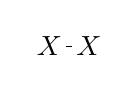
\begin{tikzpicture}[baseline={([yshift=-.5ex]current bounding box.center)}]
	\path (0,0) node (A) {$X$} ++ (0.5,0) node (B) {$X$};
	\draw (A) -- (B);
\end{tikzpicture}
\end{align}

We choose a particular 1-element set $\{*\}$ that acts as the identity in the sense that $\{*\}\times A=A\times \{*\} = A$ for any set $A$. The erase map $\text{del}_X:X\kto \{*\}$ defined by $(\text{del}_X)_x^* = 1$ is a Markov kernel that ``discards the input'' (we will later use it for marginalising joint distributions). It is drawn as a fuse:

\begin{align}
	\text{del}_X&:=\begin{tikzpicture}[baseline={([yshift=-.5ex]current bounding box.center)}]
	\path (0,0) ++ (1,0) node (B) {$X$};
	\draw[-{Rays[n=8]}] (A) -- (B);
\end{tikzpicture}
\end{align}

The copy map $\text{copy}_X:X\kto X\times X$ defined by $(\text{copy}_X)_x^{x',x''}=\llbracket x=x' \rrbracket \llbracket x=x'' \rrbracket$ is a Markov kernel that makes two identical copies of the input. It is drawn as a fork:

\begin{align}
	\text{copy}_X&:=\begin{tikzpicture}[baseline={([yshift=-.5ex]current bounding box.center)}]
	\path (0,0) node (A) {$X$} 
	++ (0.5,0) node[copymap] (copy0) {}
	++ (0.5,0.15) node (B) {$X$}
	+ (0,-0.3) node (C) {$X$};
	\draw (A) -- (copy0) to [out=45,in=180] (B) (copy0) to [out=-45, in=180] (C);
\end{tikzpicture}
\end{align}

The swap map $\text{swap}_{X,Y}:X\times Y\kto Y\times X$ defined by $(\text{swap}_{X,Y})_{x,y}^{y',x'}=\llbracket x=x' \rrbracket\llbracket y=y' \rrbracket$ swaps two inputs, and is represented by crossing wires:

\begin{align}
	\text{swap}_X &:=  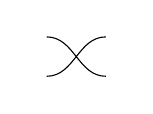
\begin{tikzpicture}[baseline={([yshift=-.5ex]current bounding box.center)}]
		\path (0,0) node (A) {} 
		+ (0,-0.5) node (B) {}
		++ (1,0) node (C) {}
		+ (0,-0.5) node (D) {};
		\draw (A) to [out=0,in=180] (D) (B) to [out=0, in=180] (C);
	\end{tikzpicture}
\end{align}

Because we anticipate that the graphical notation will be unfamiliar to many, we will also include translations to more familiar notation.

\subsection{Truncated factorisation with string diagrams}

The Markov kernels introduced in the previous section can be though of as ``conditional probability distributions without variables''. We can use these to represent an operation very similar to Equation \ref{eq:truncated_fac}. Note that $P^{\RV{Y|XZ}}$ must be represented by a Markov kernel $\kernel{K}:X\times Z\kto Y$ and $\prob{P}^{\RV{Z}}$ by a Markov kernel $\kernel{L}\in \Delta(Z)$. Then we can define a Markov kernel $\kernel{M}:X\kto X\times Z$ representing $x\mapsto \prob{P}^{\RV{YZ}}_{x}(y,z)$ by

\begin{align}
	\kernel{M}:= \tikzfig{truncated_factorisation}\label{eq:tfac_setted}
\end{align}

There is, however, a key difference between Equation \ref{eq:tfac_setted} and Equation \ref{eq:truncated_fac}: the Markov kernels in the latter equation describe the distribution of particular variables, while the former equation describes Markov kernels only.

To illustrate why we need variables, consider an arbitrary Markov kernel $\kernel{K}:\{*\}\kto \Delta(X\times X)$. We could draw this:
\begin{align}
	\kernel{K}:= \tikzfig{double_label}\label{eq:double_label}
\end{align}
We label both wires with the set $X$. However, say $X=\{0,1\}$. Then $\kernel{K}$ could be the kernel $\kernel{K}^{x_1,x_2} = \llbracket x_1 = 0\rrbracket \llbracket x_2 = 1\rrbracket$. In this case, both of its outputs must represent \emph{different} variables, despite taking values in the same set. On the other hand, if $\kernel{K}^{x_1,x_2} = 0.5 \llbracket x_1 = x_2 \rrbracket$ then both outputs coudl represent the same variable, because they are deterministically the same, or they could represent different variables that happen to be equal. We need some way to distinguish the two cases.

We use a definition of variable that almost matches the standard definition we introduced at the beginning of the section. We use Markov kernels rather than functions as it makes the construction slightly simpler.

\begin{definition}[Variable]
Given a \emph{sample space} $\Omega$ and a measurable function $f:\Omega\to A$, the variable $\RV{X}:\Omega\kto A$ induced by $f$ is the Markov kernel defined by $\RV{X}_x^a=\llbracket a = f(x) \rrbracket$.
\end{definition}

We then need a notion of Markov kernels that ``map between variables''. An \emph{indexed Markov kernel} is such an object.

\begin{definition}[Indexed Markov kernel]
Given variables $\RV{X}:\Omega\to A$ and $\RV{Y}:\Omega\to B$, an indexed Markov kernel $\kernel{K}:\RV{X}\kto \RV{Y}$ is a triple $(\kernel{K}',\RV{X},\RV{Y})$ where $\kernel{K}':A\kto B$ is the \emph{underlying kernel}, $\RV{X}$ is the \emph{input index} and $\RV{Y}$ is the \emph{output index}. Indexed Markov kernels must satisfy the property of \emph{non-contradiction}:
\begin{align}
	\max_{\omega\in \Omega} (\RV{X}\otimes\RV{Y})_{\omega,\omega}^{a',b'} = 0 \implies \kernel{K}'_{a'}^{b'} = 0
\end{align}
\end{definition}

Non-contradiction means that, if there is no $\omega\in \Omega$ such that $\RV{X}_\omega^{a'} = 1$ and $\RV{Y}_\omega^{b'}=1$ then the simultaneous occurrence of $a'$ and $b'$ must be zero.

\begin{itemize}
	\item \textbf{Product:} Given variables $\RV{W}=A\times X$ and $\RV{V}=B\times Y$, the product is $\RV{W}\otimes\RV{V}=(A\times B)\times (X\times Y)$
\end{itemize}


\subsection{Markov variable maps}\label{sec:labeled_kernels}

We will call the morphisms of our category of variables \emph{Markov variable maps}. A Markov variable map $\model{K}:\RV{A}\to \Delta(\RV{B})$ is defined by a triple $(\kernel{K}^U,\RV{A},\RV{B})$, and can be thought of as a Markov kernel that maps between variables rather than between sets of values. If $\RV{A}$ takes values in $X$ and $\RV{B}$ takes values in $Y$, we define $\kernel{K}$ as follows for all $x\in X$, $y\in Y$:

\begin{align}
	\kernel{K}_{\RV{A},x}^{\RV{B},y}  = \kernel{K}^{U y}_x
\end{align}

We call $\kernel{K}^U:X\to \Delta(Y)$ the \emph{underlying Markov kernel}.

Suppose we have Markov variable maps $\kernel{K}:\RV{A}\to \Delta(\RV{B})$ and $\kernel{L}:\RV{C}\to \Delta(\RV{D})$. Then $\kernel{K}=\kernel{L}$ iff $\RV{A}= \RV{C}$ and $\RV{B}= \RV{D}$ and $\kernel{K}^U=\kernel{L}^U$.

Given $\kernel{K}:\RV{A}\to \Delta(\RV{B})$ and $\kernel{L}:\RV{B}\to \Delta(\RV{C})$, the product $\kernel{K}\kernel{L}$ is given by

\begin{align}
	\kernel{K}\kernel{L} = (\kernel{K}^U\kernel{L}^U,\RV{A},\RV{C})
\end{align}

Note that we don't allow products of Markov variable maps if they have compatible value sets but different variables. Going back to our example of viewing variables as questions, this can be thought of as disallowing the product of a variable map that answers the question ``will this coin land heads?'' with a variable map that depends on the answer to the question ``am I taller than my brother?''.

The diagrams representing Markov variable maps are identical to the diagrams representing their underlying Markov kernels decorated with variable names on each input and each output wire. 

\todo[inline]{Show that these induce a symmetric monoidal category.}

\begin{lemma}[Deterministic equality]

\end{lemma}

A variable could be a product of other variables, e.g. $\RV{X}=\bigotimes_{i\in [n]} \RV{X}_i$. By construction, this means that we have a collection of variables $\RV{X}_i$ such that $(\RV{X}_i)_{i\in [n]}$ is the variable name associated with the product $\bigotimes_{i\in [n]} \RV{X}_i$. If each $\RV{X}_i$ takes values in a set $X_i$, then $(\RV{X}_i)_{i\in [n]}$ must take values in $\bigtimes_{i\in [n]} X_i$. The underlying Markov kernel can always be drawn with one wire representing each $X_i$, and using such a representation it is possible to assign each $\RV{X}_i$ in the sequence to a corresponding wire.

For example, if $\kernel{K}:(\RV{A}_1,\RV{A}_2)\to \Delta(\RV{B}_1,\RV{B}_2)$, for example, we can draw:

\begin{align}
	\kernel{K} := \begin{tikzpicture}[baseline={([yshift=-.5ex]current bounding box.center)}]
	\path (0,0) node (A1) {$\RV{A}_1$}
	+ (0,-0.3) node (A2) {$\RV{A}_2$}
	++ (0.7,-0.15) node[kernel] (K) {$\kernel{K}$}
	++ (0.7,0.15) node (B1) {$\RV{B}_1$}
	+ (0,-0.3) node (B2) {$\RV{B}_2$};
	\draw (A1) -- ($(K.west) + (0,0.15)$) (A2) -- ($(K.west) + (0,-0.15)$);
	\draw (B1) -- ($(K.east) + (0,0.15)$) (B2) -- ($(K.east) + (0,-0.15)$);
\end{tikzpicture}
\end{align}

or

\begin{align}
	\kernel{K} = \begin{tikzpicture}[baseline={([yshift=-.5ex]current bounding box.center)}]
	\path (0,0) node (A1) {$(\RV{A}_1,\RV{A}_2)$}
	++ (1.3,0) node[kernel] (K) {$\kernel{K}[\model{L}]$}
	++ (1.3,0.) node (B1) {$(\RV{B}_1,\RV{B}_2)$};
	\draw (A1) -- (K) -- (B1);
\end{tikzpicture}
\end{align}

\begin{lemma}[Deterministic equality of identical variables]
This axiom is equivalent to the following three conditions:

Given $\kernel{K}:(\RV{X},\RV{Y})\to \Delta(\RV{X},\RV{Z})$, there exists some $\kernel{H}:X\times Z\to \Delta(Y)$ such that
\begin{align}
	\kernel{K} &= \begin{tikzpicture}[baseline={([yshift=-.5ex]current bounding box.center)}]
					\path (0,0) node (X) {$\RV{X}$}
					+ (0,-0.65) node (Z) {$\RV{Z}$}
					++ (0.5,0) node[copymap] (copy0) {}
					++ (0.7,-0.5) node[kernel] (L) {$\kernel{H}$}
					++ (0.9,0.65) node (Xout) {$\RV{X}$}
					+  (0,-0.65) node (Y) {$\RV{Y}$};
					\draw (X) -- (copy0) to [out=-45,in=180] ($(L.west) + (0,0.15)$) (L) -- (Y);
					\draw (copy0) to [out=45,in=180] (Xout);
					\draw (Z) -- ($(L.west) + (0,-0.15)$);
				 \end{tikzpicture}\label{eq:extn1}\\
	 	&\iff\\
	 \kernel{K}_{xz}^{x'y} &= \llbracket x=x'\rrbracket \kernel{H}_{xz}^{y}
\end{align}

Given $\kernel{L}: \RV{Z}\to \Delta(\RV{X},\RV{X},\RV{Y})$, we require that there exist some $\kernel{G}:\RV{Z}\to \Delta(\RV{X}, \RV{Y})$ such that
\begin{align}
	\kernel{L} &= \begin{tikzpicture}[baseline={([yshift=-.5ex]current bounding box.center)}]
					\path (0,0) node (Z) {$\RV{Z}$}
					++ (0.9,0) node[kernel] (L) {$\kernel{G}$}
					++ (0.9,0.15) node[copymap] (copy0) {}
					++ (0.5,0.3) node (X1) {$\RV{X}$}
					++ (0,-0.3) node (X2) {$\RV{X}$}
					++  (0,-0.3) node (Y) {$\RV{Y}$};
					\draw ($(L.east) + (0,0.15)$) -- (copy0) to[out=0,in=180] (X2);
					\draw (copy0) to [out=45,in=180] (X1);
					\draw (Z)--(L) ($(L.east) + (0,-0.15)$) -- (Y);
				 \end{tikzpicture}\label{eq:extn2}\\
			   &\iff\\
		\kernel{L}_{z}^{xx'y} &= \llbracket x=x' \rrbracket\kernel{G}_{z}^{xy}	   
\end{align}

There is no $\kernel{M}:(\RV{X},\RV{X},\RV{Y})\to \Delta(\RV{W},\RV{Z})$.
\end{lemma}

\begin{proof}
Suppose some variable $\RV{X}$ appears 
\end{proof}

\todo[inline]{If the category of variables and Markov variable maps is symmetric monoidal..}

There is a natural isomorphism between two Markov variable maps  $\kernel{K}$ and $\kernel{L}$ if one can be obtained from the other by application of a sequence of swaps. For example, if we have $\kernel{K}:(\RV{X},\RV{Y})\to \Delta(\RV{Z},\RV{W})$ and $\kernel{L}:(\RV{Y},\RV{X})\to \Delta(\RV{W},\RV{Z})$, then $\kernel{K}\cong \kernel{L}$ if

\begin{align}
\tikzfig{equivalence}
\end{align}

\subsection{Connection}

Connection is an associative operation $\rightrightarrows$ that ``joins'' two labeled Markov kernels where the labels can be matched and preserves unmatched inputs and outputs. A key property of connection is that, if both input Markov kernels satisfy Axiom 1, then the output also satisfies axiom 1. One can think of this operation like connecting two lego bricks of different sizes -- we connect all the parts that will fit together, and all the connection points that don't fit are left available.

For some variable $\RV{W}$, we use $m_{\RV{W}}(\RV{X})$ to refer to the number of times $\RV{W}$ appears in $\RV{X}$ (recalling that $\RV{X}$ may be a sequence of other variables). We say $\RV{W}$ is in $\RV{X}$ or $\RV{W}\in \RV{X}$ if $m_{\RV{W}}(\RV{X})>0$.

With this in mind, we define the following operations on sequences of labels

\begin{enumerate}
	\item \textbf{Difference of label sequences:} Given $\RV{X}_1$, $\RV{X}_2$, the difference $\RV{X}_1\setminus \RV{X}_2$ is a variable $\RV{X}_3$ such that for all variables $\RV{W}_i$, $m_{\RV{W}_i}(\RV{X}_3) = \max(0,m_{\RV{W}_i}(\RV{X}_1)-m_{\RV{W}_i}(\RV{X}_2))$
	\item \textbf{Intersection of labels:} Given $\RV{X}_1$, $\RV{X}_2$, the intersection $\RV{X}_1\cap \RV{X}_2$ is a variable $\RV{X}_3$ such that for any variable $\RV{W}_i$, $m_{\RV{W}_i}(\RV{X}_3) = \min(m_{\RV{W}_i}(\RV{X}_1),m_{\RV{W}_i}(\RV{Y}_2))$
\end{enumerate}

These definitions are non-unique in that they do not define the order of the resulting label sequence. This doesn't cause a problem because we only care about Markov variable maps that are identical up to isomorphism.

Given two Markov variable maps $\kernel{F}:\RV{I}_F\to\Delta(\RV{O}_F)$ and $\kernel{S}:\RV{I}_S\to\Delta(\RV{O}_S)$, make the following variable identifications:
\begin{align}
	\RV{O}_{F\cdot}&:=\RV{O}_F\setminus\RV{I}_S &\text{Variables only in the output of } \kernel{F}\\
	\RV{O}_{FS}&:=\RV{O}_F\cap\RV{I}_S &\text{Variables in the output of both}\\
	\RV{I}_{F\cdot} &:= \RV{I}_F\setminus \RV{I}_S &\text{Variables only in the input } \kernel{F}\\
	\RV{I}_{FS}&:= \RV{I}_F\cap\RV{I}_S &\text{Variables in the input of both}\\
	\RV{I}_{\cdot S}&:= \RV{I}_S\setminus \RV{I}_F &\text{Variables only in the input of }\kernel{S} \\
	\RV{O}_{I_FO_S*}&:=\RV{O}_S\cap \RV{I}_F\setminus \RV{I}_S &\text{Input of }\kernel{F}\text{ and the output only of }\kernel{S}\\
	\RV{O}_{O_FO_S*} &:= \RV{O}_F\cap\RV{O}_S\setminus \RV{I}_S&\text{Output of }\kernel{F}\text{ and the output only of }\kernel{S}\\
\end{align}

$\kernel{F}$ can be connected to $\kernel{S}$ iff $\RV{O}_{I_FO_S*}$ synonymous with $*$ and $\RV{O}_{O_FO_S*}$ is also synonymous with $*$. The reason for this is that, in general, if these sets were non-empty then we would not have a way to connect $\kernel{F}$ and $\kernel{S}$ without violating the deterministic equality of identical variables.

\begin{definition}[connection]\label{def:extension}
Consider a labeled Markov kernel $\kernel{F}:\RV{I}_F\to\Delta(\RV{O}_F)$ which can be connected to $\kernel{S}:\RV{I}_S\to\Delta(\RV{O}_S)$. Because they can be conected, we can write $\kernel{F}:(\RV{I}_{F\cdot},\RV{I}_{FS})\to\Delta(\RV{O}_{F\cdot},\RV{O}_{FS}))$ and $\kernel{S}:(\RV{I}_{FS},\RV{I}_{\cdot S})\to\Delta(\RV{O}_S)$.

Then Equations \ref{eq:extn_definition1} and \ref{eq:extn_definition2} are equivalent definitions of connection:
\begin{align}
	\kernel{K}\rightrightarrows \kernel{L} &:=  \begin{tikzpicture}[baseline={([yshift=-.2ex]current bounding box.center)}]
		\path (0,0) node (Y) {$\RV{I}_{F\cdot}$}
		+ (0,-0.3) node (Q) {$\RV{I}_{FS}$}
		+ (0,-0.8) node (R) {$\RV{I}_{\cdot S}$}
		++ (0.5,-0.3) node[copymap] (copy0) {}
		++ (0.5,0.15) node[kernel] (K) {$\kernel{F}$}
		++ (0.5,-0.15) node[copymap] (copy1) {}
		++ (0.6,-0.5) node[kernel] (L) {$\kernel{S}$}
		++ (0.6, 0.8) node (Z) {$\RV{O}_{F\cdot}$}
		+ (0,-0.3) node (X) {$\RV{O}_{FS}$}
		+ (0,-0.8) node (W) {$\RV{O}_S$};
		\draw (Y) -- ($(K.west) + (0,0.15)$) (Q) -- ($(K.west) + (0,-0.15)$);
		\draw (copy0) to [out=-45,in=180] ($(L.west) + (0,0)$) (copy1) to [out=-60,in=180] ($(L.west) + (0,0.15)$);
		\draw (R) to [out=0,in=180] ($(L.west) + (0,-0.15)$);
		\draw ($(K.east) + (0,-0.15)$) to (copy1);
		\draw ($(K.east) + (0,0.15)$) -- (Z) (copy1) to [out=0,in=180] (X) (L) -- (W);
	\end{tikzpicture}\label{eq:extn_definition1}\\
	&:= \kernel{J}\\
	\kernel{J}_{yqr}^{zxw} &= \kernel{F}_{yq}^{zx} \kernel{S}_{xqr}^{w}\label{eq:extn_definition2}
\end{align}
Note that there are no sums in Equation \ref{eq:extn_definition1}, this is simply a product of matrix elements.
\end{definition}

\begin{lemma}[Connection is associative up to permuation of labels]\label{lem:con_associative}
Given labeled Markov kernels $\kernel{K}:\RV{I}_K\to\Delta(\RV{O}_K)$, $\kernel{L}:\RV{I}_L\to\Delta\RV{O}_L)$ and $\kernel{J}:\RV{I}_J\to\Delta(\RV{O}_J)$,
\begin{align}
	(\kernel{K}\rightrightarrows \kernel{L})\rightrightarrows \kernel{J} &\overset{perm}{=} \kernel{K}\rightrightarrows (\kernel{L}\rightrightarrows \kernel{J})
\end{align}
\end{lemma}

\begin{proof}
Proven in Appendix \ref{sec:connect_associative}
\end{proof}

\begin{lemma}[Identity maps commute one way with connection]
Consider the identity map on some labeled set $\kernel{I}:\RV{X}\to \Delta(\RV{X})$ (note that by Equation \ref{eq:extn1} the identity map is the \emph{only} kernel with this signature). For any $\kernel{M}:\RV{Y}\to\Delta(\RV{Z})$, either a copy of $\RV{X}$ appears in the output but not the input and $\kernel{I}\rightrightarrows \kernel{M}$ is undefined, or $\kernel{I}\rightrightarrows\kernel{M}=\kernel{M}\rightrightarrows\kernel{I}$.
\end{lemma}

\begin{proof}
Consider the identity map on some labeled set $\kernel{I}:\RV{X}\to \Delta(\RV{X})$ (note that by Equation \ref{eq:extn1} the identity map is the \emph{only} kernel with this signature). Note that for any $\kernel{M}:\RV{Y}\to\Delta(\RV{Z})$, either a copy of $\RV{X}$ appears in the output but not the input, in which case $\kernel{I}\rightrightarrows \kernel{M}$ is undefined, or we have one of the following cases:

If $\RV{X}$ is in $\RV{Y}$ and $\RV{Z}$, then there must be some $\kernel{N}$ such that Equation \ref{eq:extn1} holds. Defining $\RV{Y}'=\RV{Y}\setminus\RV{X}$ and $\RV{Z}'=\RV{Z}\setminus\RV{X}$:

\begin{align}
	\kernel{I}\rightrightarrows\kernel{M}&=\tikzfig{iconnectm}\\
										 &=\tikzfig{iconnectm_rev}\\
										 &=\kernel{M}\rightrightarrows\kernel{I}
\end{align}

\todo[inline]{Commutativity of copy map in appendix}

If $\RV{X}$ is in $\RV{Y}$ only, defining $\RV{Y}'=\RV{Y}\setminus\RV{X}$:

\begin{align}
	\kernel{I}\rightrightarrows\kernel{M}&=\tikzfig{iconnectm_clear}\\
										 &=\kernel{M}\rightrightarrows\kernel{I}
\end{align}

If $\RV{X}$ is in neither $\RV{Y}$ nor $\RV{Z}$, then

\begin{align}
	\kernel{I}\rightrightarrows\kernel{M}&=\tikzfig{iconnectm_dclear}\\
										 &=\kernel{M}\rightrightarrows\kernel{I}
\end{align}
\end{proof}

\begin{theorem}[Connection is compatible with axiom 1]
Given $\kernel{K}:\RV{A}\to\Delta(\RV{B})$ and $\kernel{L}:\RV{C}\to\Delta(\RV{D})$, let $\kernel{J}=\kernel{K}\rightrightarrows \kernel{L}$. Then $\kernel{J}$ satisfies axiom 1.
\end{theorem}

\begin{proof}
By inspecting the definition of $\rightrightarrows$ (Equation \ref{eq:extn_definition1}), we can see that no labels from either of the inputs are increased in multiplicity. We need to verify that if either of the inputs has a label with multiplicity $>1$, then the result of the extension still satisfies axiom 1. 

Consider any label $\RV{X}$ that appears in both the input and output of $\kernel{K}$, or twice in the output of $\kernel{K}$. Then Equation \ref{eq:extn3} implies that there exists some $\kernel{H}$ such that $\kernel{K}=\kernel{H}\rightrightarrows\kernel{I}$.

Thus

\begin{align}
	\kernel{K}\rightrightarrows \kernel{L} &= (\kernel{H}\rightrightarrows \kernel{I})\rightrightarrows\kernel{L}\\
										   &\overset{perm}{=} \kernel{H}\rightrightarrows(\kernel{I}\rightrightarrows\kernel{L})\\
										   &= \kernel{H}\rightrightarrows(\kernel{L}\rightrightarrows\kernel{I})\\
										   &\overset{perm}{=} (\kernel{H}\rightrightarrows\kernel{L})\rightrightarrows\kernel{I}
\end{align}

Which implies that $\kernel{J}$ satistfies Equation \ref{eq:extn3} for $\RV{Y}$.

Consider $\RV{Z}$ that appears in the input and output of $\kernel{L}$ or twice in the output of $\kernel{L}$. Then there exists some $\kernel{G}$ such that

\begin{align}
	\kernel{K}\rightrightarrows \kernel{L} &= \kernel{K}\rightrightarrows (\kernel{G}\rightrightarrows\kernel{I})\\
										   &\overset{perm}{=} (\kernel{K}\rightrightarrows \kernel{G})\rightrightarrows\kernel{I}
\end{align}

Which implies $\kernel{J}$ satisfies Equation \ref{eq:extn3}.
\end{proof}

\subsection{Submodels}

Note that at this point, we have a theory of probability that can handle Equation \ref{eq:truncated_fac}. In particular, $P^{\RV{Y|XZ}}$ must be represented by a Markov variable map $\kernel{K}:(\RV{X}, \RV{Z})\to \Delta(\RV{Y})$ and $\prob{P}^{\RV{Z}}$ by a Markov variable map $\kernel{L}\in \Delta(\RV{Z})$. Then we can define a Markov variable map $\kernel{M}:\RV{X}\to \Delta(\RV{X}, \RV{Z})$ representing $x\mapsto \prob{P}^{\RV{YZ}}_{x}(y,z)$ by

\begin{align}
	\kernel{M}&:= \kernel{L}\rightrightarrows\kernel{K}\\
	 		&=\tikzfig{truncated_factorisation_labeled}\label{eq:tfac_labeled}
\end{align}

We can see that Equation \ref{eq:tfac_labeled} is almost identical to Equation \ref{eq:tfac_setted} except with set labels instead of sets annotating the wires. This minor change, along with Axiom 1, deals with the problem of identical sets previously mentioned.

However, we do not yet have a notion of \emph{marginal probability} or \emph{conditional probability}. In the paragraph above, the terms $P^{\RV{Y|XZ}}$ and $\prob{P}^{\RV{Z}}$ are external to the theory developed so far. However, we do know that they are related in a particular way; namely, they are respectively a contitional distribution and a marginal distribution derived from the same probability space with measure $P$. 

We will use the term \emph{submodels} to refer to marginals and conditionals of a higher level model, like those mentioned in the previous paragraph. 

\begin{definition}[Marginal]
For any label $\RV{X}$, define the marginalising kernel $\text{del}_{\RV{X}}:\RV{X}\to *$, which is necessarily unique. Given $\kernel{K}:\RV{W}\to\Delta(\RV{Y})$ and $\kernel{L}:\RV{W}\to \Delta(\RV{Z})$, $\RV{L}$ is a \emph{marginal} of $\kernel{K}$ if, for some $\RV{X}$ in $\RV{Y}$,
\begin{align}
	\kernel{K}\rightrightarrows\text{del}_{\RV{X}} = \kernel{L}
\end{align}
\end{definition}

Because $\kernel{K}\rightrightarrows \text{del}_*=\kernel{K}$, $\kernel{K}$ is always a marginal of itself.

\begin{definition}[Submodel]
Given $\kernel{K}:\RV{X}\to \Delta(\RV{Y})$ and $\kernel{L}:\RV{W}\to\Delta(\RV{Z})$, $\kernel{L}$ is a submodel of $\kernel{K}$ if there are marginals $\kernel{K}'$, $\kernel{K}''$ of $\kernel{K}$ such that
\begin{align}
	 \kernel{K}'\rightrightarrows\kernel{L} = \kernel{K}''
\end{align}
\end{definition}

As the trivial map $\text{del}_*:\RV{X}\to\Delta(\{*\})$ is a marginal of $\kernel{K}$, and $\text{del}_*\rightrightarrows\kernel{K}'=\kernel{K}'$ for any marginal of $\kernel{K}$, every marginal of $\kernel{K}$ is also a submodel of $\kernel{K}$.

With the definition of submodels in hand, we can introduce a notation more familiar to people experienced with probability theory. If $\kernel{L}:\RV{X}\to \Delta(\RV{Y})$ is a submodel of $\kernel{K}$, we may write $\kernel{L}\equiv \kernel{K}^{\RV{Y}|\RV{X};\kernel{L}}$ and $\kernel{L}_x^y\equiv \kernel{K}^{\RV{Y}|\RV{X};\kernel{L}}(y|x)$. Note that the same kernel might be a submodel of many other kernels. This notation isn't \emph{entirely} familiar, as we retain a reference to the original kernel $\kernel{L}$. In general, a kernel $\kernel{K}$ has many submodels with the same signature, and this non-uniqueness is more problematic for causal models than for standard probabilistic models, as we will see in Section \ref{sec:CBN}.

However, we will sometimes write $\model{K}^{\RV{Y}|\RV{X}}=\model{L}^{\RV{Y}|\RV{X}}$. This means that some $\kernel{Q}$ exists such that $\model{K}^{\RV{Y}|\RV{X};\kernel{Q}}=\model{L}^{\RV{Y}|\RV{X};\kernel{Q}}$; alternatively, $\kernel{Q}$ is a submodel of $\model{K}$ and $\model{L}$.

\begin{lemma}[Submodel existence]\label{lem:subm_exist}
In FinStoch, for any $\kernel{K}:\RV{W}\to \Delta(\RV{X},\RV{Y})$ there exists a submodel $\model{K}^{\RV{Y}|\RV{XW};\kernel{L}}$.
\end{lemma}

\begin{proof}
Consider any Markov kernel $\kernel{L}:(\RV{X},\RV{W})\to \Delta(\RV{Y})$ with the property
\begin{align}
	\kernel{L}_{xw}^{y} = \frac{\kernel{K}_w^{xy}}{\sum_{x\in X}\kernel{K}_w^{xy}}\qquad\forall {w,y}:\text{ the denominator is positive}
\end{align}

Then define $\kernel{K}^{\RV{X}|\RV{W};\kernel{M}}:=\kernel{K}\rightrightarrows\text{del}_{\RV{Y}}$, which is a marginal of $\kernel{K}$. THen
\begin{align}
	(\kernel{M}\rightrightarrows\kernel{L})_w^{xy} &= \kernel{M}_w^x\kernel{L}_{xw}^y&\\
												   &= \sum_{x\in X} \kernel{K}_w^{xy} \frac{\kernel{K}_w^{xy}}{\sum_{x\in X}\kernel{K}_w^{xy}} &\text{ if }\kernel{K}_w^{xy}>0\\
												   &= \kernel{K}_w^{xy} &\text{ if }\kernel{K}_w^{xy}>0\\
												   &= 0 &\text{otherwise}\\
												   &= \kernel{K}_w^{xy} &\text{otherwise}
\end{align}
\end{proof}

We did not use string diagrams in this proof, so this result does not necessarily apply to other Markov kernel categories. This is the technical reason why we choose to work with FinStoch: the existence of submodels presents a challenge in more general settings that we haven't fully resolved and the progress we have is beyond the scope of this paper.

\subsection{Conditional independence}\label{ssec:cond_indep}

We define conditional independence in the following manner:

For a \emph{probability distribution} $\kernel{P}:\{*\}\to \Delta(\RV{Y})$ and some $\RV{A},\RV{B},\RV{C}\in \RV{Y}$, we say $\RV{A}$ is independent of $\RV{B}$ given $\RV{C}$, written $\RV{A}\CI_{\kernel{P}}\RV{B}|\RV{C}$, if there are submodels $\model{P}^{\RV{ABC};\kernel{J}}$, $\model{P}^{\RV{C};\kernel{K}}$, $\model{P}^{\RV{A}|\RV{C};\kernel{L}}$, $\model{P}^{\RV{B}|\RV{C};\kernel{M}}$ such that

\begin{align}
	\kernel{P}^{\RV{ABC};\kernel{J}} &= \tikzfig{cond_indep1}
\end{align}

For a \emph{kernel} $\kernel{N}:\RV{X}\to \Delta(\RV{Y})$ and some $\RV{A},\RV{B},\RV{C}\in (\RV{X},\RV{Y})$, we say $\RV{A}$ is independent of $\RV{B}$ given $\RV{C}$, written $\RV{A}\CI_{\kernel{N}}\RV{B}|\RV{C}$, if there is some $\kernel{O}:\{*\}\to \Delta(\RV{X})$ such that $O^x>0$ for all $x\in X$ and $\RV{A}\CI_{\kernel{O}\rightrightarrows\kernel{N}} \RV{B}|\RV{C}$.

This definition is inappliccable in the case where sets may be uncountably infinite, as no such $\kernel{O}$ can exist in this case. There may well be definitions of conditional independence that generalise better, and we refer to the discussions in \citet{fritz_synthetic_2020} and \citet{constantinou_extended_2017} for some discussion of alternative definitions. One advantage of this definition is that it matches the version given by \citet{cho_disintegration_2019} which they showed coincides with the standard notion of conditional independence and so we don't have to show this in our particular case.

A particular case of interest is when a kernel $\kernel{K}:(\RV{X},\RV{W})\to \Delta(\RV{Y})$ can, for some $\kernel{L}:\RV{W}\to \Delta(\RV{Y})$, be written:

\begin{align}
	\kernel{K} = \tikzfig{ci_example}
\end{align}

Then $\RV{Y}\CI_{\kernel{K}}\RV{W}|\RV{X}$.

\subsection{Variables or vague variables?}\label{sec:vague_variables}

Recall our definition of variables: functions from a sample space $\Omega$ to some codomain set. We also recall a concern raised in our introduction: if actions affecting a measure of interest are vague, then potential outcome random variables \emph{might} be ill-defined. Consider: how can it be that the degree to which we specify actions sometimes, but not always, allows a random variable to be well-defined? These concerns seem to be of different types -- on the one hand, we have the problem of whether my instructions are clear enough for you to follow them and produce the same results, and on the other hand the problem of whether an abstract sample space has the appropriate properties for a certain type of function to exist.

Consider also the definition of \emph{variable} found in \citet{pearl_causality:_2009}:

\begin{quote}
By a \emph{variable} we will mean an attribute, measurement or inquiry that may take on one of several possible outcomes, or values, from a specified domain. If we have beliefs (i.e., probabilities) attached to the possible values that a variable may attain, we will call that variable a random variable.
\end{quote}

This is claimed to be identical to our definition of a variable -- i.e. a measurable function on the sample space. However, we feel that a much closer match is the definition of a \emph{qualitative statistical random variable} given by \citet{menger_random_2003}; roughly speaking, a qualitative statistical random variable is a vague function (our term) whose codomain is well-specified but whose domain is not. Menger offers examples of vague functions that take as arguments acts of measurement, or people in Chicago; in a very similar manner, Pearl's definition offers examples of arguments that a variable may take, but does not offer examples of sample spaces that may form their domains.

We offer the following rough idea of how vague random variables can be thought about. A vague random variable like ``$\RV{X}$ represents whether this coin lands on heads or tails'' can be considered an instruction for whoever is reading to construct a concrete random variable whose domain is related to the set of observations that they might receive. These domains necessarily differ between individuals, and we postulate the existence of a ``reality'' that offers everyone observations that are sometimes similar in some respects. A vague random variable can be well-defined if the concrete random variables that everyone constructs allow everyone to agree on the result when they are given observations that are appropriately related.

This might seem an excessively pedantic way to describe a coin-flipping experiment. However, we think there that a story like this this may be important in causal models. At the start of this section we asked ``how can the degree to which we specify actions sometimes, but not always, allows a random variable to be well-defined?'' Our rough model of vague variables offers a solution to this question: sufficiently specific actions are sometimes enough to allow all parties to agree on the values once observations have taken place. We hypothesise that this question arises with variables representing consequences of actions because when it comes to taking actions there is an asymmetry that is extremely hard to avoid: I know more about what I am doing and why I am doing it than you do.

While we believe that this is a potentially fruitful line of inquiry, we won't develop it here and will satisfy ourselves with a theory based on concrete variables.